% Source of the figure transformations.pdf: the three transformations of a pseudo-square with terminals a, b, c, d
% along a cut {e_1, e_2} of two edges (thick dashed arrows); the state before is on the left, the state after on
% the right. (a) Both edges lie inside the square. (b) One edge lies inside. (c) No edge lies inside.
% Compile with pdfLaTeX; the PDF is included in the manuscript at its natural size.
\documentclass[tikz,border=1pt]{standalone}
\usepackage[T1]{fontenc}
\pdfinfoomitdate=1 \pdftrailerid{} \pdfsuppressptexinfo=-1
\usetikzlibrary{arrows.meta,shapes.geometric}
\definecolor{fblue}{RGB}{31,102,178}
\tikzset{
  every node/.append style={text=black},
  vertex/.style={circle, fill=black, inner sep=0pt, minimum size=2.2mm},
  terminal/.style={circle, fill=black, inner sep=0pt, minimum size=3mm},
  square/.style={rounded corners=4pt, fill=gray!10, draw=gray!75!black, line width=0.9pt},
  part/.style={rounded corners=5pt, fill=gray!30, draw=gray!70, line width=0.6pt},
  link/.style={ellipse, fill=gray!32, draw=gray!75!black, line width=0.6pt, inner sep=0pt,
               minimum width=9mm, minimum height=6mm},
  fedge/.style={line width=0.9pt, fblue, dash pattern=on 3pt off 1.6pt, -{Stealth[length=2.4mm, width=2mm]}},
  cutedge/.style={fedge, line width=1.7pt, dash pattern=on 4pt off 2pt},
  becomes/.style={line width=1pt, -{Stealth[length=3mm, width=2.6mm]}}}
\begin{document}
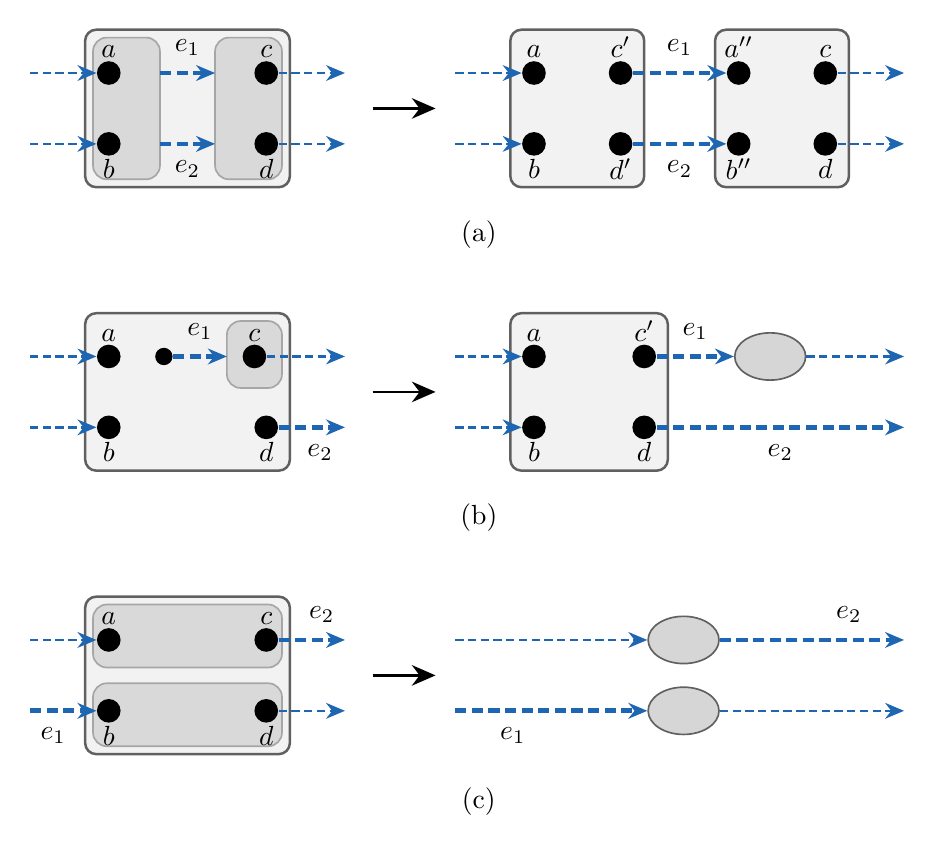
\begin{tikzpicture}[x=1cm, y=1cm]
  \def\X{5.4}  % left end of the state after the transformation
  % ---------------- (a): both edges inside the square ----------------
  \begin{scope}
    \draw[square] (0,-1) rectangle (2.6,1);
    \draw[part] (0.1,-0.9) rectangle (0.95,0.9);
    \draw[part] (1.65,-0.9) rectangle (2.5,0.9);
    \node[terminal] (a)  at (0.3,0.45)  {};
    \node[terminal] (b)  at (0.3,-0.45) {};
    \node[terminal] (c)  at (2.3,0.45)  {};
    \node[terminal] (d)  at (2.3,-0.45) {};
    \node[above=2pt] at (a) {$a$};
    \node[below=2pt] at (b) {$b$};
    \node[above=2pt] at (c) {$c$};
    \node[below=2pt] at (d) {$d$};
    \draw[fedge] (-0.7,0.45) -- (a);
    \draw[fedge] (-0.7,-0.45) -- (b);
    \draw[fedge] (c) -- (3.3,0.45);
    \draw[fedge] (d) -- (3.3,-0.45);
    \draw[cutedge] (0.95,0.45) -- (1.65,0.45) node[midway, above=2pt] {$e_1$};
    \draw[cutedge] (0.95,-0.45) -- (1.65,-0.45) node[midway, below=2pt] {$e_2$};
    \draw[becomes] (3.65,0) -- (4.45,0);
    % after: two squares joined by two single-edge general paths
    \draw[square] (\X,-1) rectangle (\X+1.7,1);
    \draw[square] (\X+2.6,-1) rectangle (\X+4.3,1);
    \node[terminal] (a1) at (\X+0.3,0.45)  {};
    \node[terminal] (b1) at (\X+0.3,-0.45) {};
    \node[terminal] (c1) at (\X+1.4,0.45)  {};
    \node[terminal] (d1) at (\X+1.4,-0.45) {};
    \node[terminal] (a2) at (\X+2.9,0.45)  {};
    \node[terminal] (b2) at (\X+2.9,-0.45) {};
    \node[terminal] (c2) at (\X+4.0,0.45)  {};
    \node[terminal] (d2) at (\X+4.0,-0.45) {};
    \node[above=2pt] at (a1) {$a$};
    \node[below=2pt] at (b1) {$b$};
    \node[above=2pt] at (c1) {$c'$};
    \node[below=2pt] at (d1) {$d'$};
    \node[above=2pt] at (a2) {$a''$};
    \node[below=2pt] at (b2) {$b''$};
    \node[above=2pt] at (c2) {$c$};
    \node[below=2pt] at (d2) {$d$};
    \draw[fedge] (\X-0.7,0.45) -- (a1);
    \draw[fedge] (\X-0.7,-0.45) -- (b1);
    \draw[fedge] (c2) -- (\X+5.0,0.45);
    \draw[fedge] (d2) -- (\X+5.0,-0.45);
    \draw[cutedge] (c1) -- (a2) node[midway, above=2pt] {$e_1$};
    \draw[cutedge] (d1) -- (b2) node[midway, below=2pt] {$e_2$};
    \node at (5.0,-1.6) {(a)};
  \end{scope}
  % ---------------- (b): one edge inside the square ----------------
  \begin{scope}[yshift=-3.6cm]
    \draw[square] (0,-1) rectangle (2.6,1);
    \draw[part] (1.8,0.05) rectangle (2.5,0.9);
    \node[vertex]   (t)  at (1.0,0.45)  {};
    \node[terminal] (a)  at (0.3,0.45)  {};
    \node[terminal] (b)  at (0.3,-0.45) {};
    \node[terminal] (c)  at (2.15,0.45) {};
    \node[terminal] (d)  at (2.3,-0.45) {};
    \node[above=2pt] at (a) {$a$};
    \node[below=2pt] at (b) {$b$};
    \node[above=2pt] at (c) {$c$};
    \node[below=2pt] at (d) {$d$};
    \draw[fedge] (-0.7,0.45) -- (a);
    \draw[fedge] (-0.7,-0.45) -- (b);
    \draw[fedge] (c) -- (3.3,0.45);
    \draw[cutedge] (d) -- (3.3,-0.45) node[midway, below=2pt, xshift=3pt] {$e_2$};
    \draw[cutedge] (t) -- (1.8,0.45) node[midway, above=2pt] {$e_1$};
    \draw[becomes] (3.65,0) -- (4.45,0);
    % after: the square shrinks and the general path above grows by a link
    \draw[square] (\X,-1) rectangle (\X+2.0,1);
    \node[terminal] (a1) at (\X+0.3,0.45)  {};
    \node[terminal] (b1) at (\X+0.3,-0.45) {};
    \node[terminal] (c1) at (\X+1.7,0.45)  {};
    \node[terminal] (d1) at (\X+1.7,-0.45) {};
    \node[link] (lk) at (\X+3.3,0.45) {};
    \node[above=2pt] at (a1) {$a$};
    \node[below=2pt] at (b1) {$b$};
    \node[above=2pt] at (c1) {$c'$};
    \node[below=2pt] at (d1) {$d$};
    \draw[fedge] (\X-0.7,0.45) -- (a1);
    \draw[fedge] (\X-0.7,-0.45) -- (b1);
    \draw[cutedge] (c1) -- (lk) node[midway, above=2pt] {$e_1$};
    \draw[fedge] (lk) -- (\X+5.0,0.45);
    \draw[cutedge] (d1) -- (\X+5.0,-0.45) node[midway, below=2pt] {$e_2$};
    \node at (5.0,-1.6) {(b)};
  \end{scope}
  % ---------------- (c): no edge inside the square ----------------
  \begin{scope}[yshift=-7.2cm]
    \draw[square] (0,-1) rectangle (2.6,1);
    \draw[part] (0.1,0.1) rectangle (2.5,0.9);
    \draw[part] (0.1,-0.9) rectangle (2.5,-0.1);
    \node[terminal] (a)  at (0.3,0.45)  {};
    \node[terminal] (b)  at (0.3,-0.45) {};
    \node[terminal] (c)  at (2.3,0.45)  {};
    \node[terminal] (d)  at (2.3,-0.45) {};
    \node[above=2pt] at (a) {$a$};
    \node[below=2pt] at (b) {$b$};
    \node[above=2pt] at (c) {$c$};
    \node[below=2pt] at (d) {$d$};
    \draw[fedge] (-0.7,0.45) -- (a);
    \draw[cutedge] (-0.7,-0.45) -- (b) node[pos=0.35, below=2pt] {$e_1$};
    \draw[cutedge] (c) -- (3.3,0.45) node[pos=0.65, above=2pt] {$e_2$};
    \draw[fedge] (d) -- (3.3,-0.45);
    \draw[becomes] (3.65,0) -- (4.45,0);
    % after: the square dissolves into two general paths
    \node[link] (lu) at (\X+2.2,0.45)  {};
    \node[link] (ll) at (\X+2.2,-0.45) {};
    \draw[fedge] (\X-0.7,0.45) -- (lu);
    \draw[cutedge] (lu) -- (\X+5.0,0.45) node[pos=0.7, above=2pt] {$e_2$};
    \draw[cutedge] (\X-0.7,-0.45) -- (ll) node[pos=0.3, below=2pt] {$e_1$};
    \draw[fedge] (ll) -- (\X+5.0,-0.45);
    \node at (5.0,-1.6) {(c)};
  \end{scope}
\end{tikzpicture}
\end{document}
